\section{Conceptual model}

The app has two main entities, subjects, and students, they are marked with thicker borders. 
\begin{itemize}
    \item Students are the users of the app and they can create and course subjects.
    \item Subjects are what students course that lead to an examination or qualification. A subject is taught in a faculty, and a faculty belongs to a university. Also, subjects are done in a course (usually a semester). 
    \item Faculty, university, and course are not relevant for the app's requirements, they are just related concepts, so in the database, they'll be just attributes of a subject, not standalone classes.
    \item A subject contains one or more evaluations and one or more exams. An evaluation contains exams with weights.
\end{itemize}

The main takeaway from the conceptual model (Fig. \ref{fig:conceptual-model}) is that students create and course subjects, and subjects have evaluations with exams and basic information to be searched like short name, full name, university or course. 

\vfill
\begin{figure}[ht!]
    \center
    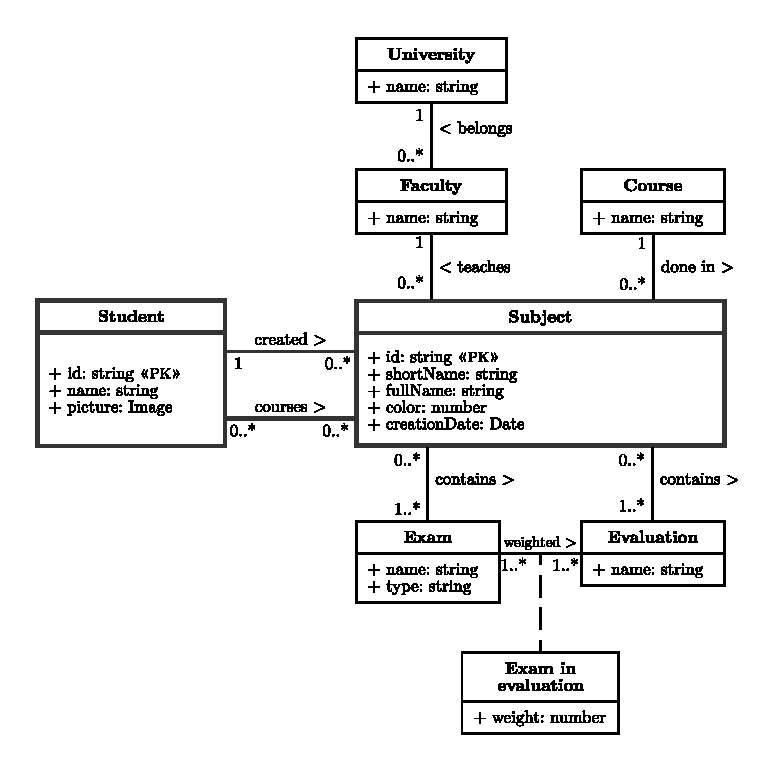
\includegraphics[width=\linewidth]{media/diagrams/conceptual.pdf}
    \caption{Conceptual model's UML Diagram}
    \label{fig:conceptual-model}
\end{figure}
\vfill
